
\documentclass[paper=a4, fontsize=11pt]{scrartcl} % A4 paper and 11pt font size

\usepackage[utf8]{inputenc}
\usepackage[spanish]{babel}

\usepackage{graphicx}
\usepackage{url}
\usepackage{amsmath,amsfonts,amsthm} % Math packages
\usepackage{sectsty} % Allows customizing section commands
%\allsectionsfont{\centering \normalfont\scshape} % Make all sections centered, the default font and small caps
\usepackage{fancyhdr} % Custom headers and footers
\pagestyle{fancyplain} % Makes all pages in the document conform to the custom headers and footers
\fancyhead{} % No page header - if you want one, create it in the same way as the footers below
\fancyfoot[L]{} % Empty left footer
\fancyfoot[C]{} % Empty center footer
\fancyfoot[R]{\thepage} % Page numbering for right footer
\renewcommand{\headrulewidth}{0pt} % Remove header underlines
\renewcommand{\footrulewidth}{0pt} % Remove footer underlines
\setlength{\headheight}{13.6pt} % Customize the height of the header

\numberwithin{equation}{section} % Number equations within sections (i.e. 1.1, 1.2, 2.1, 2.2 instead of 1, 2, 3, 4)
\numberwithin{figure}{section} % Number figures within sections (i.e. 1.1, 1.2, 2.1, 2.2 instead of 1, 2, 3, 4)
\numberwithin{table}{section} % Number tables within sections (i.e. 1.1, 1.2, 2.1, 2.2 instead of 1, 2, 3, 4)


%----------------------------------------------------------------------------------------
%   TITLE SECTION
%----------------------------------------------------------------------------------------


\title{
\normalfont \normalsize
\textsc{Facultad de Ingeniería de la Universidad de Buenos Aires} \\ [20pt] % Your university, school and/or department name(s)
\huge Trabajo Práctico de Señales y Sistemas \\ % The assignment title
}

\author{Juan Manuel Pérez} % Your name

\date{\normalsize\today} % Today's date or a custom date

\newcommand{\stft}{\emph{STFT}}

\begin{document}

\maketitle % Print the title


\section{Ejercicio 1 y 2}

Recordemos que un espectrograma es una representación visual donde se muestra el espectro de una señal en función del tiempo. Para esto, se separa el dominio del tiempo en ventanas y para cada una se aplica una Transformada de Fourier de Tiempo Corto (\stft).


La \stft tiene los siguientes parámetros:

\begin{itemize}
    \item Tipo de ventana
    \item Tamaño de ventana
    \item Step
    \item Tamaño de las FFTs
\end{itemize}

La elección de estos parámetros nos define la resolución tanto en el tiempo como en el espectro: a mayor tamaño de ventana (mayor N), menos resolución temporal y mayor resolución en las frecuencias; inversamente, si hago decrecer el N obtengo mejor resolución en el tiempo pero peor en las frecuencias.

Por lo tanto, es necesario entender el trade-off entre ambas y tomar una decisión al respecto. En nuestro caso, al estar analizando piezas de piano, nos interesa obtener una resolución en frecuencias tal que nos permita distinguir entre dos notas. Así mismo, también queremos tener una resolución temporal que nos permita distinguir temporalmente la ocurrencia de cada nota.

\subsection{Elección de parámetros}


De la tabla de frecuencias de las notas observamos que la distancia mínima entre semitono es de 31hz, con lo cuál necesitamos tener tal resolución como mínimo.

Sabemos que la DFT $X[k]$ de tamaño $N$ es un muestreo de la transformada de Fourier $X(e^{jw})$ cada $2\pi/N$. Queremos que este muestreo pueda distinguir cada 30 hz, con lo cual queremos que

\begin{equation}
 \frac{2\pi}{N} < \frac{2\pi 30}{Fs}
\end{equation}

Despejando, obtenemos que $N \geq 534$, o lo que es lo mismo, que la ventana debe ser más grande que $0.34ms$

Probamos entonces con los siguientes valores de ventana y step:

\begin{itemize}
    \item 16 ms de ventana y 8 de step
    \item 34 ms de ventana y 17 de step
    \item 100 ms de ventana y 50 de step

\end{itemize}

Podemos observar en \ref{s_16_8} que si bien obtenemos buena resolución temporal, no es posible distinguir las notas. Para las otras elecciones de parámetros (\ref{s_34_17} y \ref{s_100_50}) se distingue mucho mejor las notas, aún cuando en la última configuración perdamos cierta

Finalmente, elegimos una ventana de 100 ms ya que nos brinda mayor nitidez en las frecuencias, aún a cuesta de pérdida de resolución temporal. Podremos, en este caso, distinguir más o menos notas separadas por 100ms, es decir, 10 por segundo.

\begin{figure}[th!]
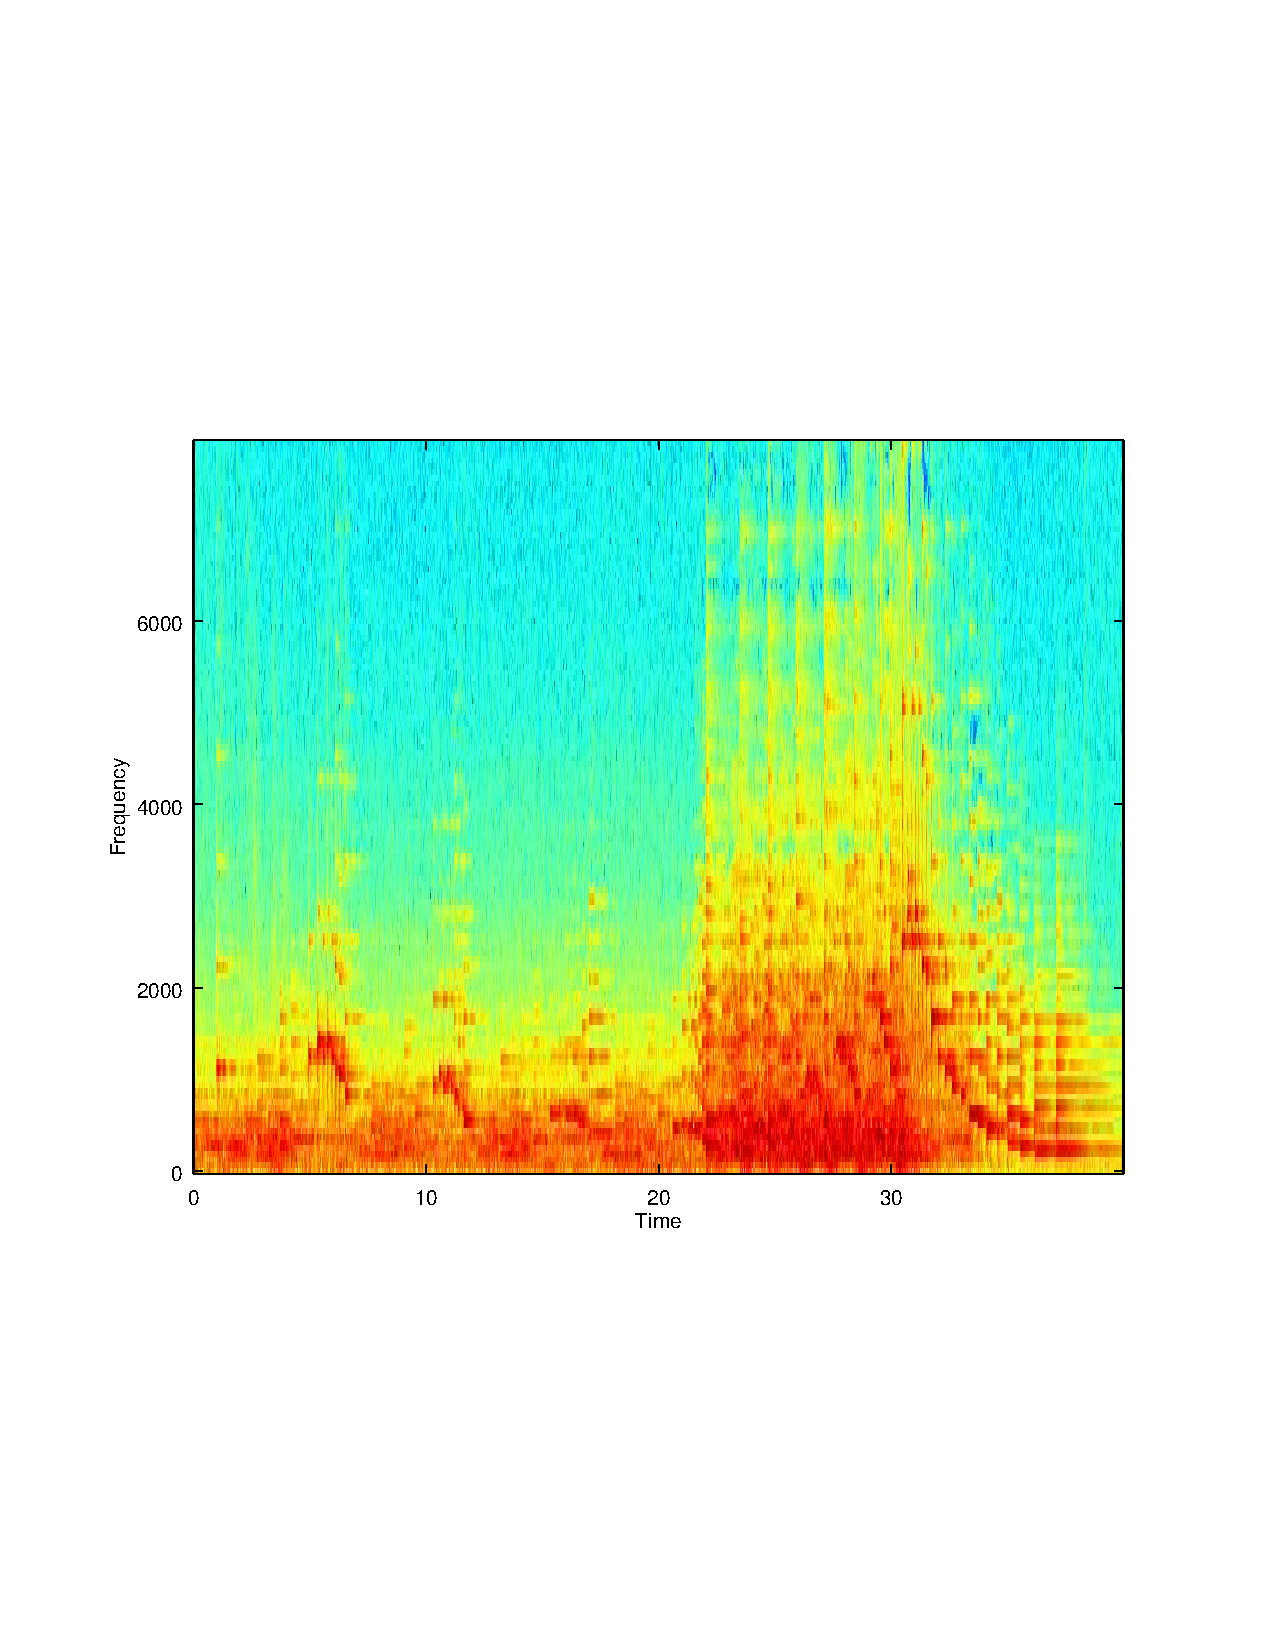
\includegraphics[width=\textwidth]{../images/specgram_w16s8.pdf}
\caption{Espectrograma de ventana 16 ms y step de 8ms}
\label{s_16_8}
\end{figure}


\begin{figure}[th!]
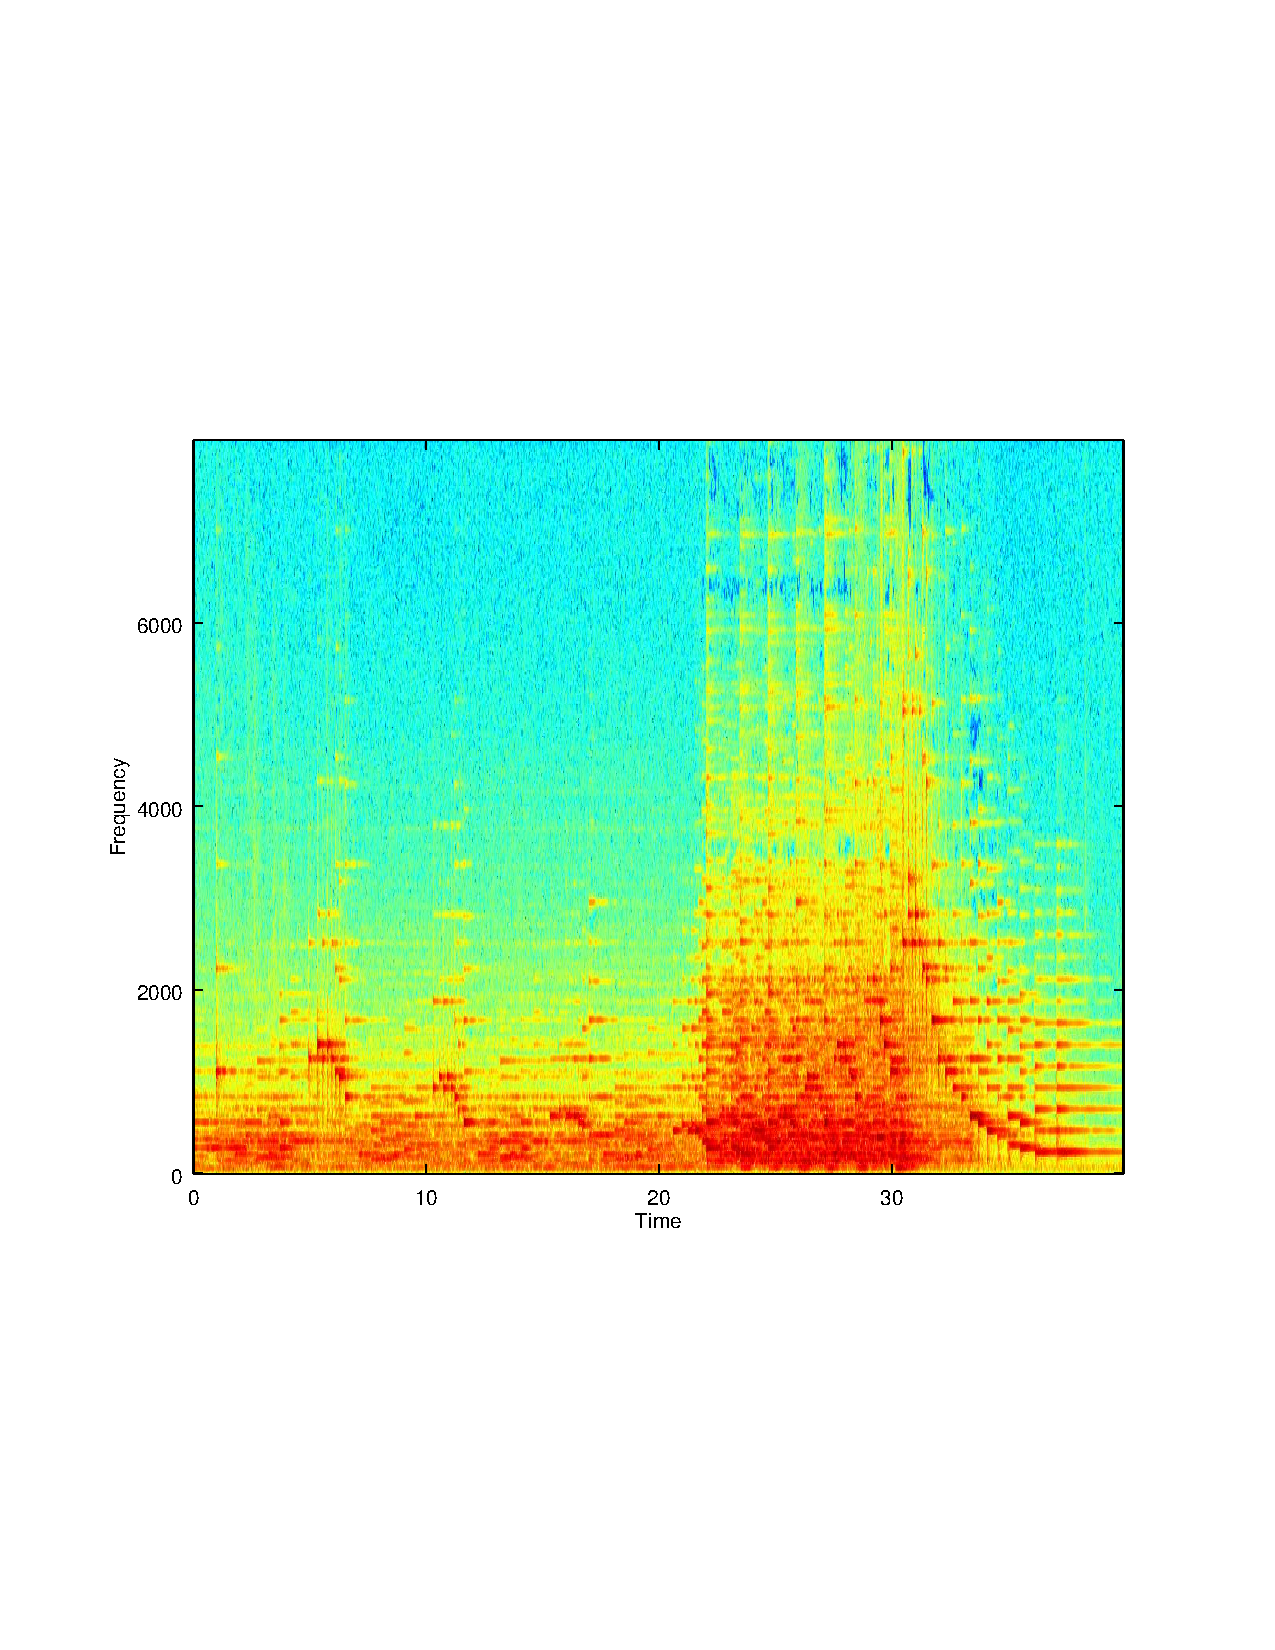
\includegraphics[width=\textwidth]{../images/specgram_w34s17.pdf}
\caption{Espectrograma de ventana 34 ms y step de 17 ms}
\label{s_34_17}
\end{figure}

\begin{figure}[th!]
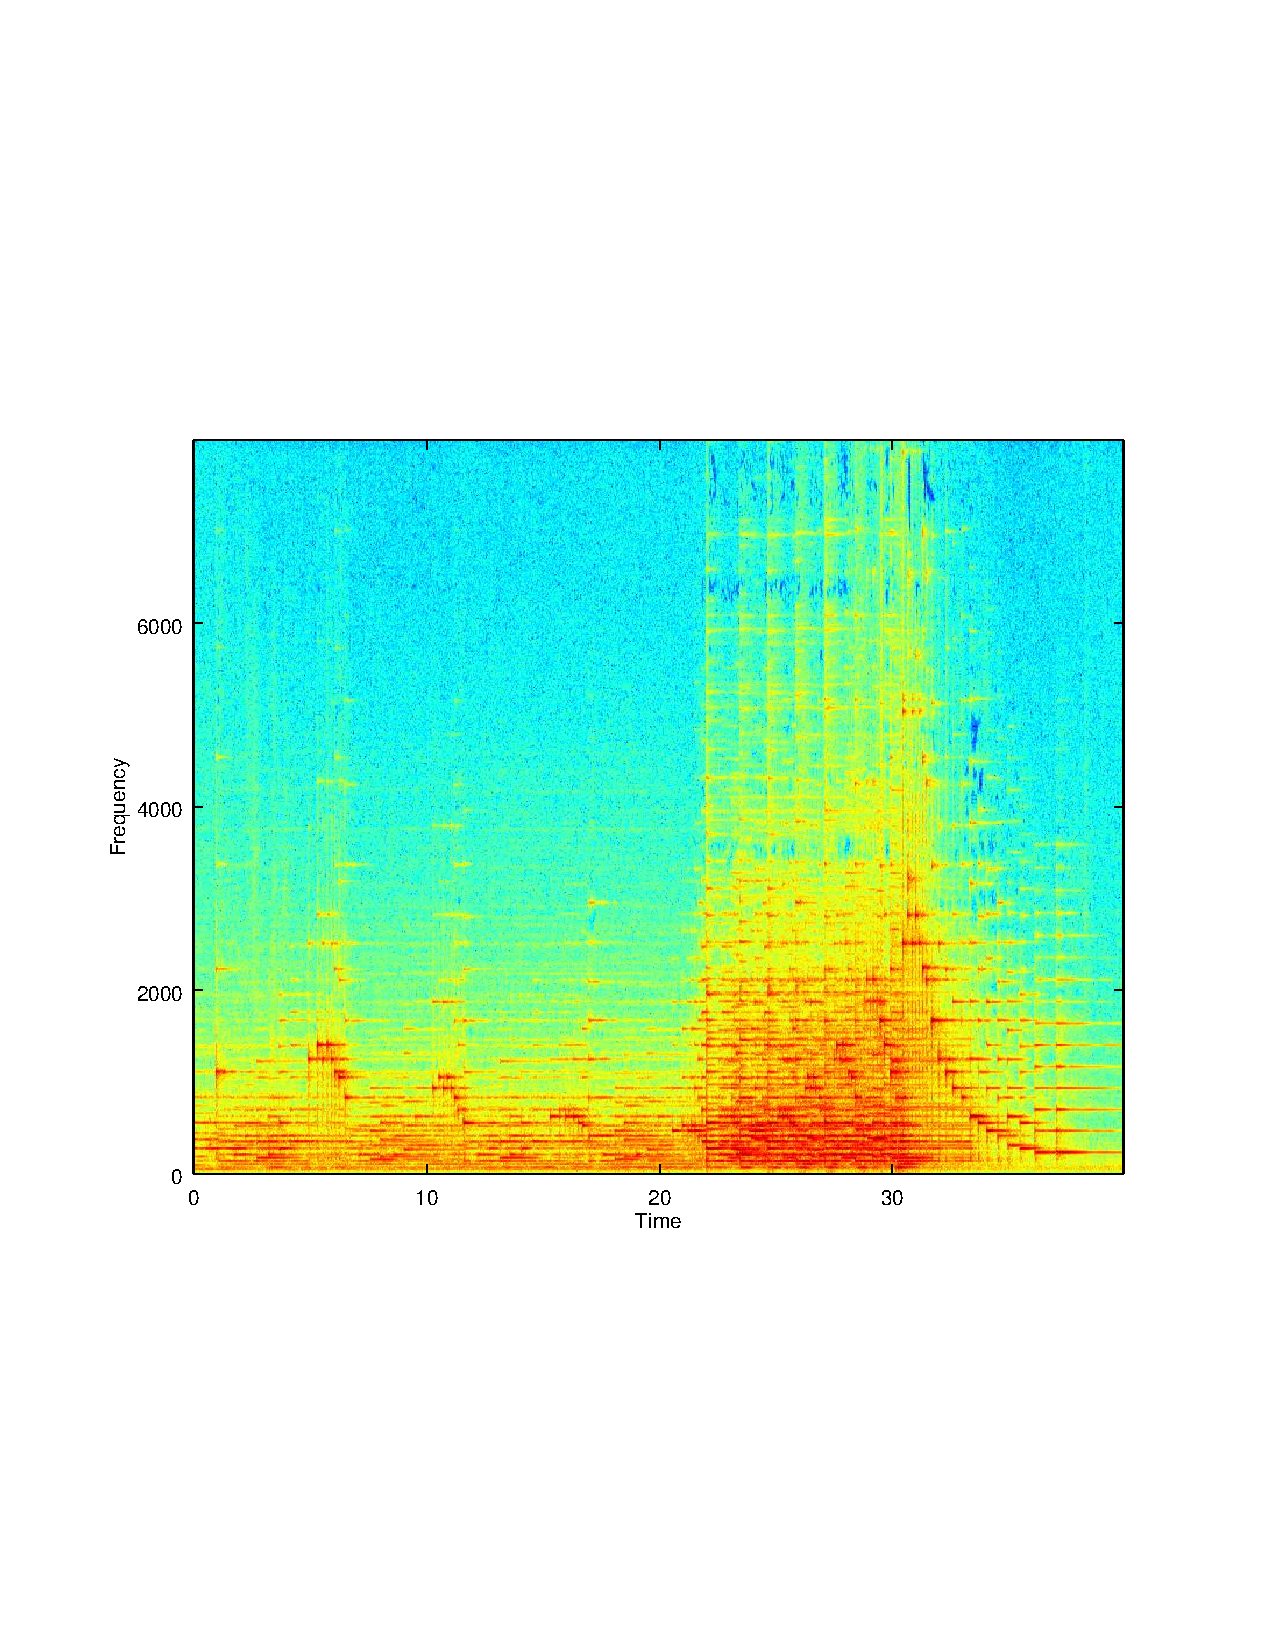
\includegraphics[width=\textwidth]{../images/specgram_w100s50.pdf}
\caption{Espectrograma de ventana 100 ms y step de 50 ms}
\label{s_100_50}
\end{figure}


\section{Ejercicio 3}

\begin{figure}[bh!]
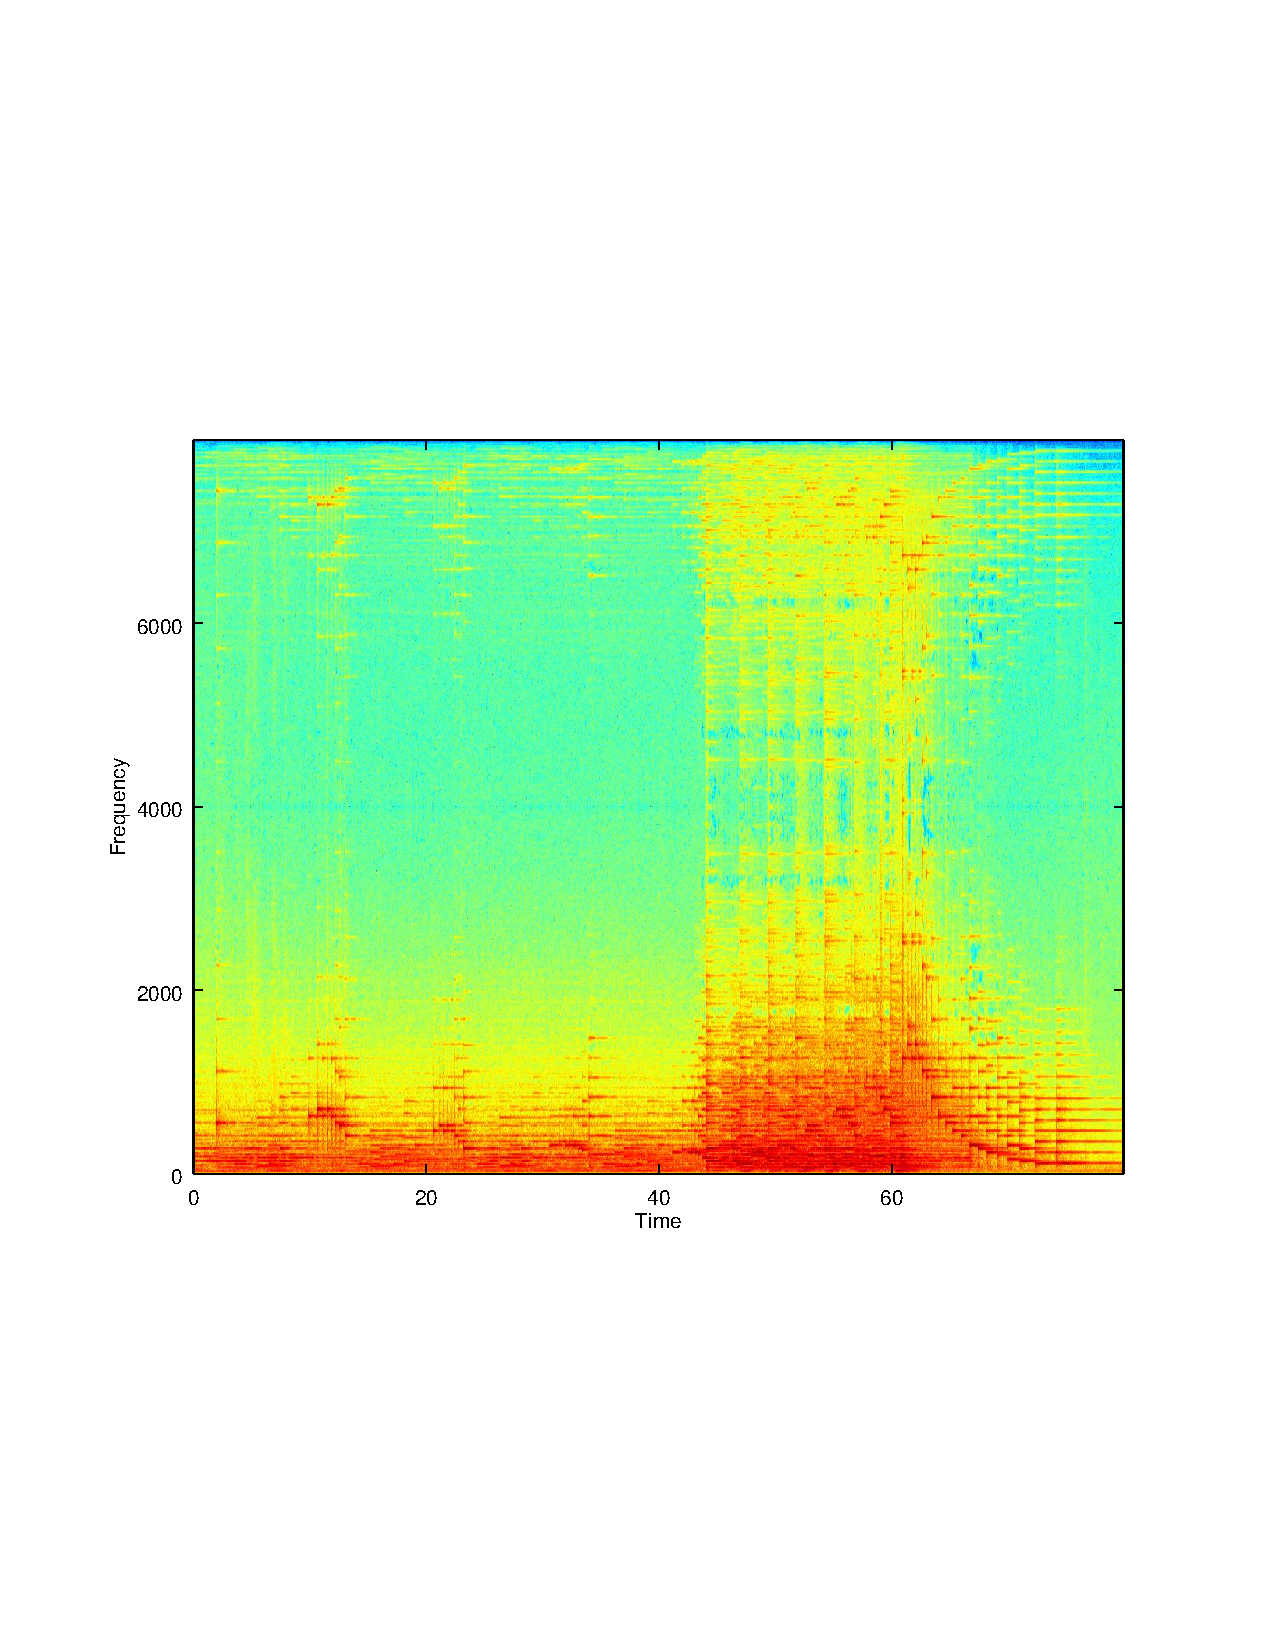
\includegraphics[width=\textwidth]{../images/specgram_3_interpolated.pdf}
\caption{Espectrograma del audio interpolado linealmente}
\label{audio_interp_lineal}
\end{figure}

En este primer intento de duplicar el largo del audio, interpolamos entre muestras del audio.

Como es de esperarse, esto baja a la mitad el pitch de cada nota, ya que podemos pensar que la onda que antes tardaba N muestras en ciclar ahora le va a tomar 2N. A su vez, la interpolación lineal agrega armónicos de alta frecuencia, como podemos observar en el espectrograma de la figura \ref{audio_interp_lineal}.


\section{Ejercicio 4}

En este punto se nos pide reducir el audio a la mitad de la duración usando una decimación de orden dos, es decir

\begin{equation}
    Y[n] = X[2n]
\end{equation}

Sabemos por propiedades de la transformada de Fourier en tiempo discreto que esto genera un ensanchamiento del espectro, con lo cuál debemos aplicar un filtro pasa bajos para evitar tener aliasing. El tipo de filtro elegido fue un Butterworth de orden 10 y frecuencia de corte $\frac{\pi}{2}$, es decir, la mitad de la frecuencia de Nyquist. La elección de este tipo de filtro se debe a que es uno de los más simples y se mantiene bastante plano hasta la frecuencia de corte.

En la figura \ref{audio_decimado} podemos observar el espectrograma. Como es de esperarse, las frecuencias de las notas se multiplican por dos (suben una octava) producto de que son reproducidas a ``mayor velocidad''.


\begin{figure}[t]
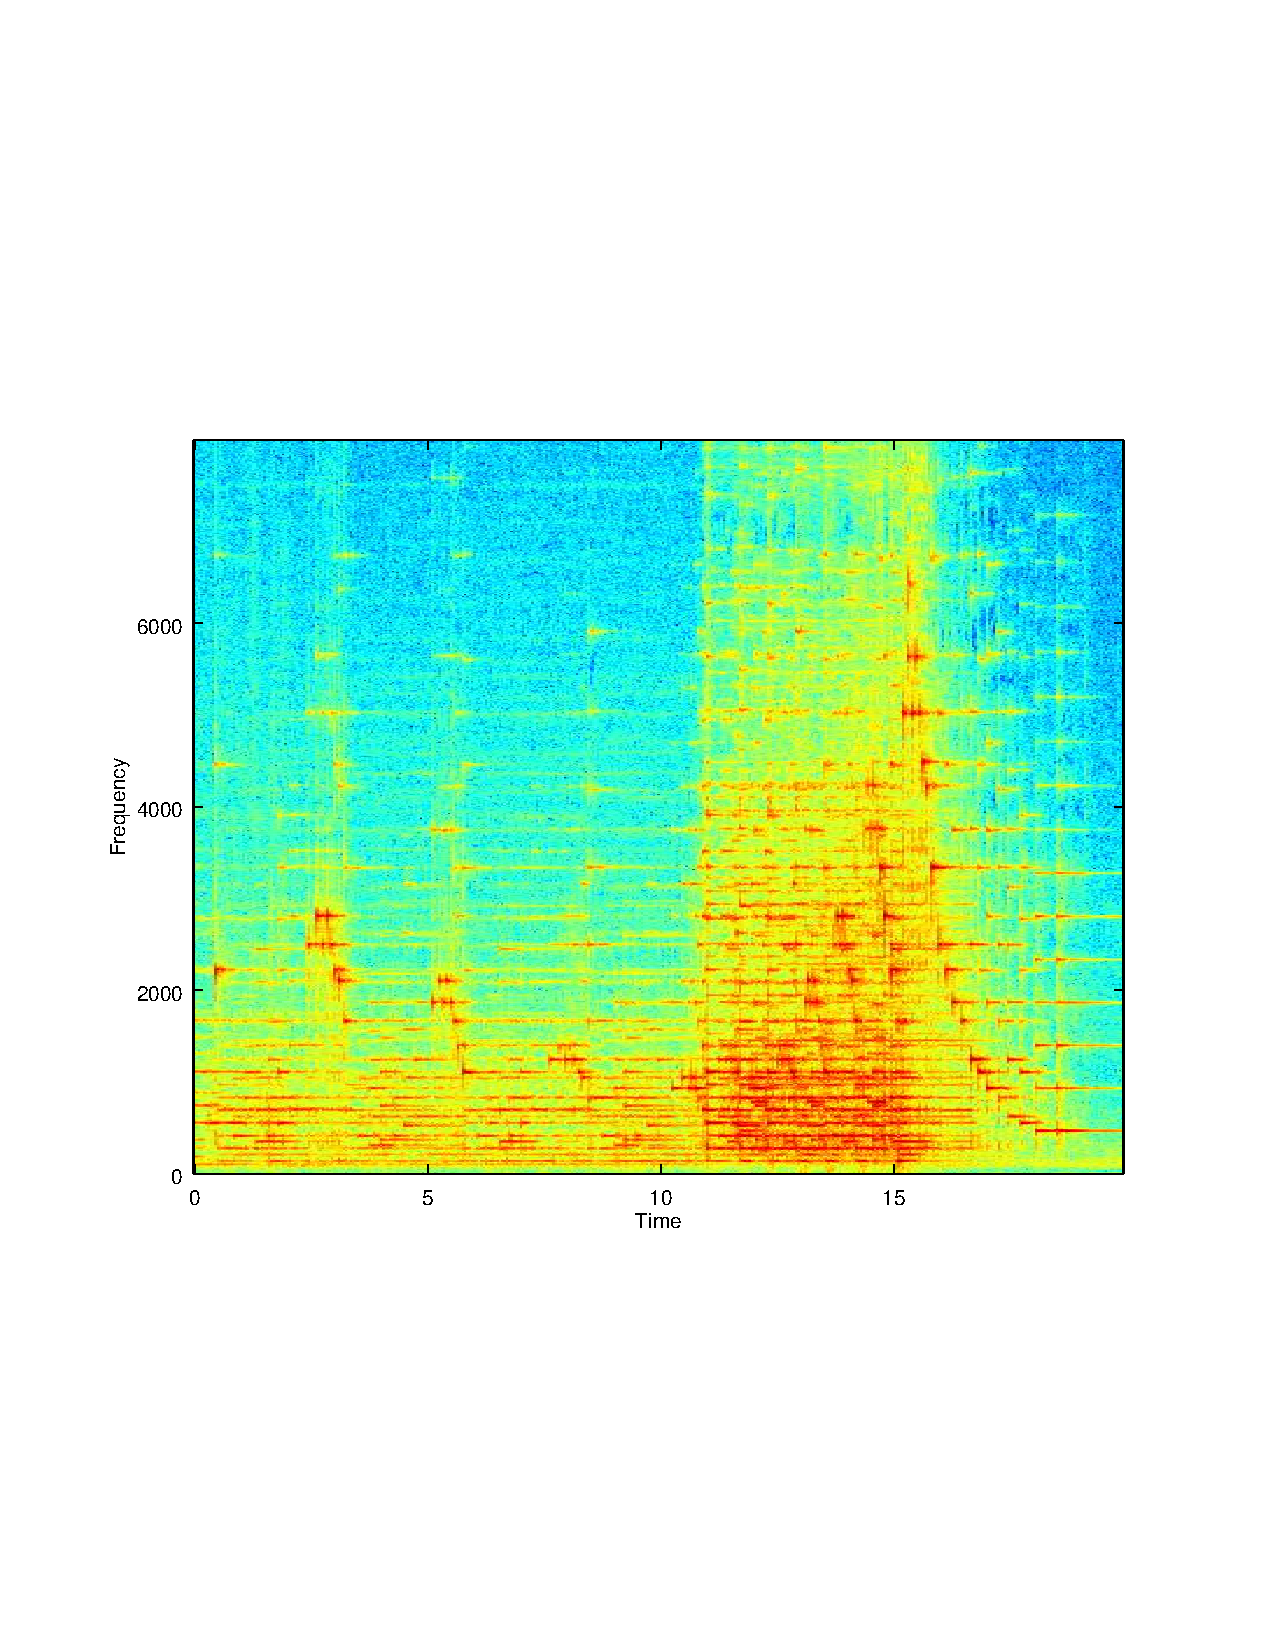
\includegraphics[width=\textwidth]{../images/specgram_4_decimated.pdf}
\caption{Espectrograma del audio decimado}
\label{audio_decimado}
\end{figure}



\section{Ejercicio 5}

Este punto nos pide reconstruir una señal en base a su espectrograma. Este problema se conoce como la transformada inversa de Fourier de tiempo corto.

En \footnote{\url{http://ieeexplore.ieee.org.sci-hub.cc/abstract/document/1455039/#}}, uno de los primeros trabajos en el área, se discuten dos alternativas para esta tarea. La que decidimos utilizar fue similar al método llamado OverLap Addition (OLA): de cada rebanada espectral, reconstruir un pedazo de la señal y luego concatenarlos.

Para esto,

\begin{itemize}
    \item Rellenamos con los conjugados simétricos
    \item Calculamos la \emph{ifft} de cada rebanada
    \item Dividimos por una ventana de \emph{hanning}
    \item Concatenamos los distintos segmentos con un offset
\end{itemize}

El último paso surgió como medida paliativa ya que notábamos que los segmentos iniciales y finales de cada pieza reconstruída resultaban sensiblemente atenuados.

En el gráfico \ref{diff_audio_reconstruido} se puede observar la diferencia entre el audio reconstruído y el audio original. En este caso, la reconstrucción es casi perfecta (salvando principio y final del audio).


\begin{figure}[t!]
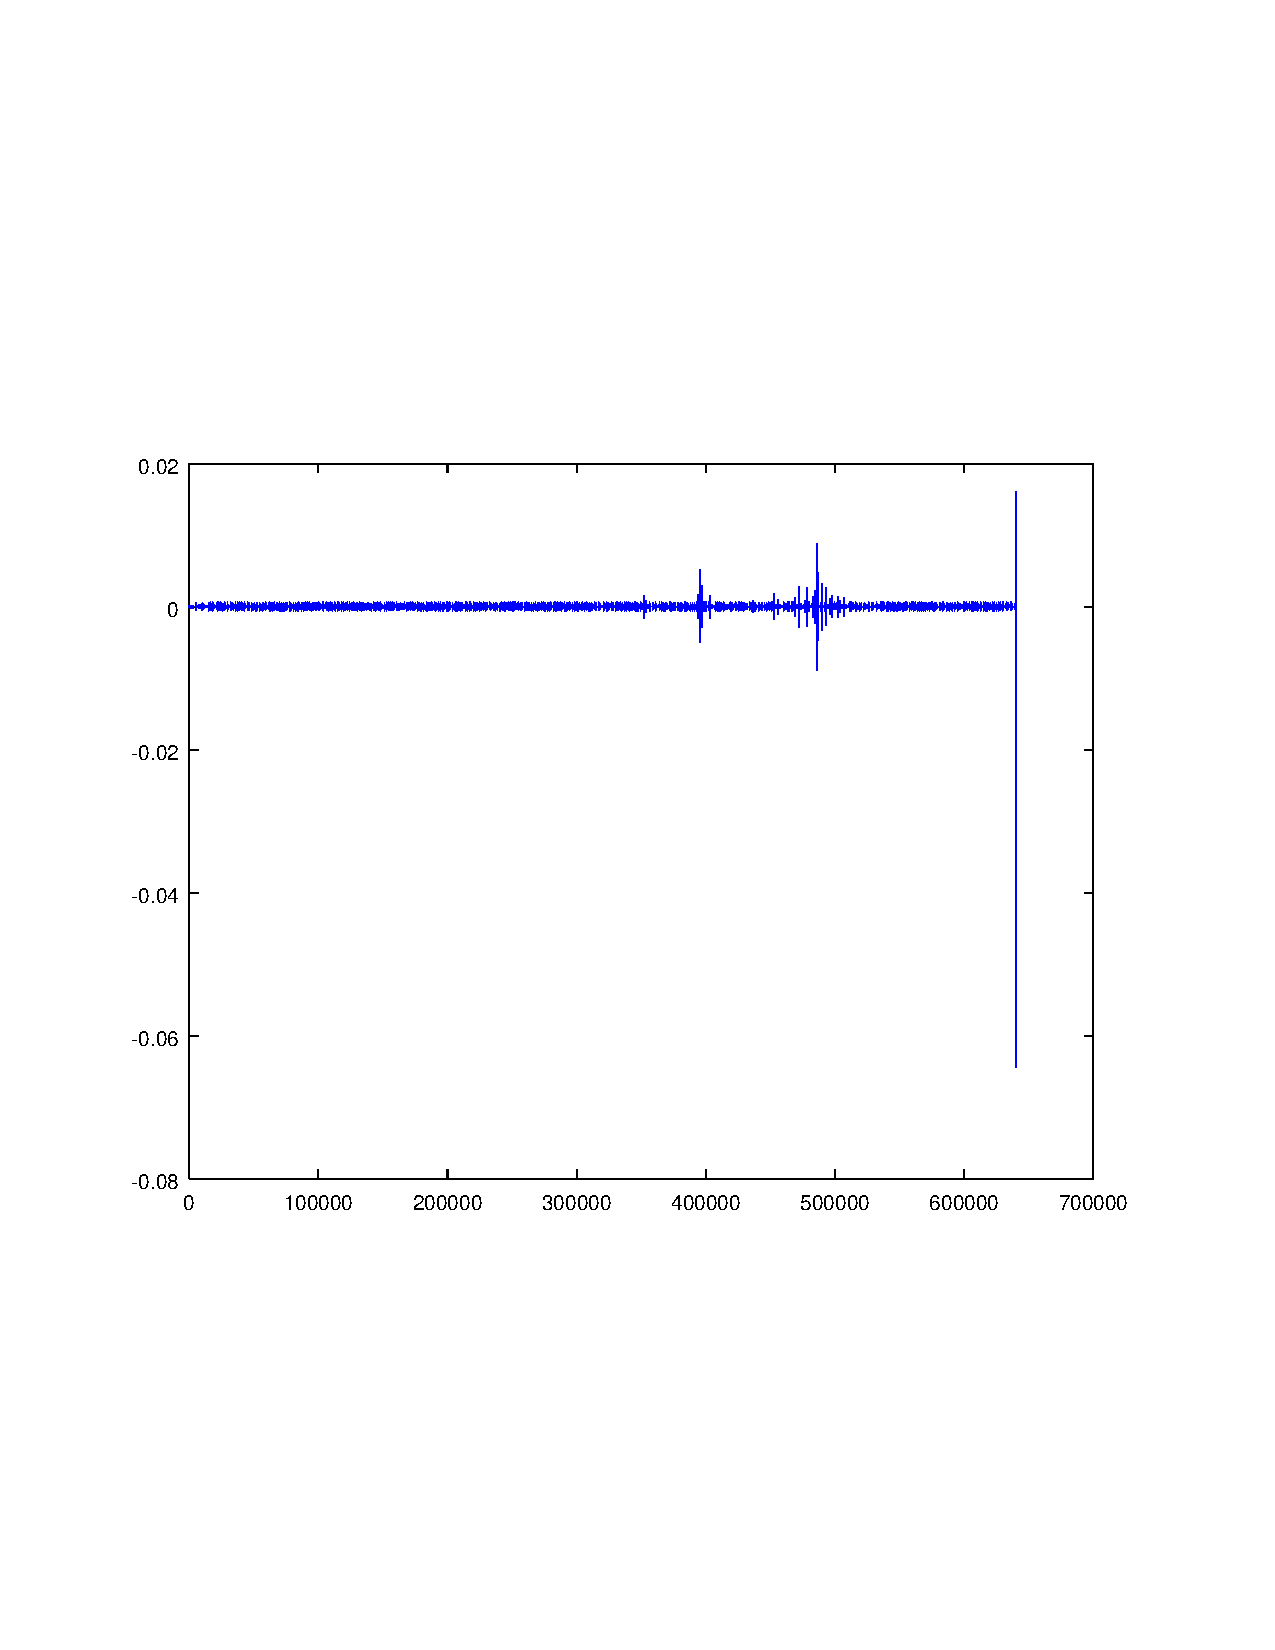
\includegraphics[width=\textwidth]{../images/difference_reconstruction_5.pdf}
\caption{Diferencia entre audio y audio reconstruído espectralmente}
\label{diff_audio_reconstruido}
\end{figure}


\section{Ejercicio 6}

\begin{figure}[t!]
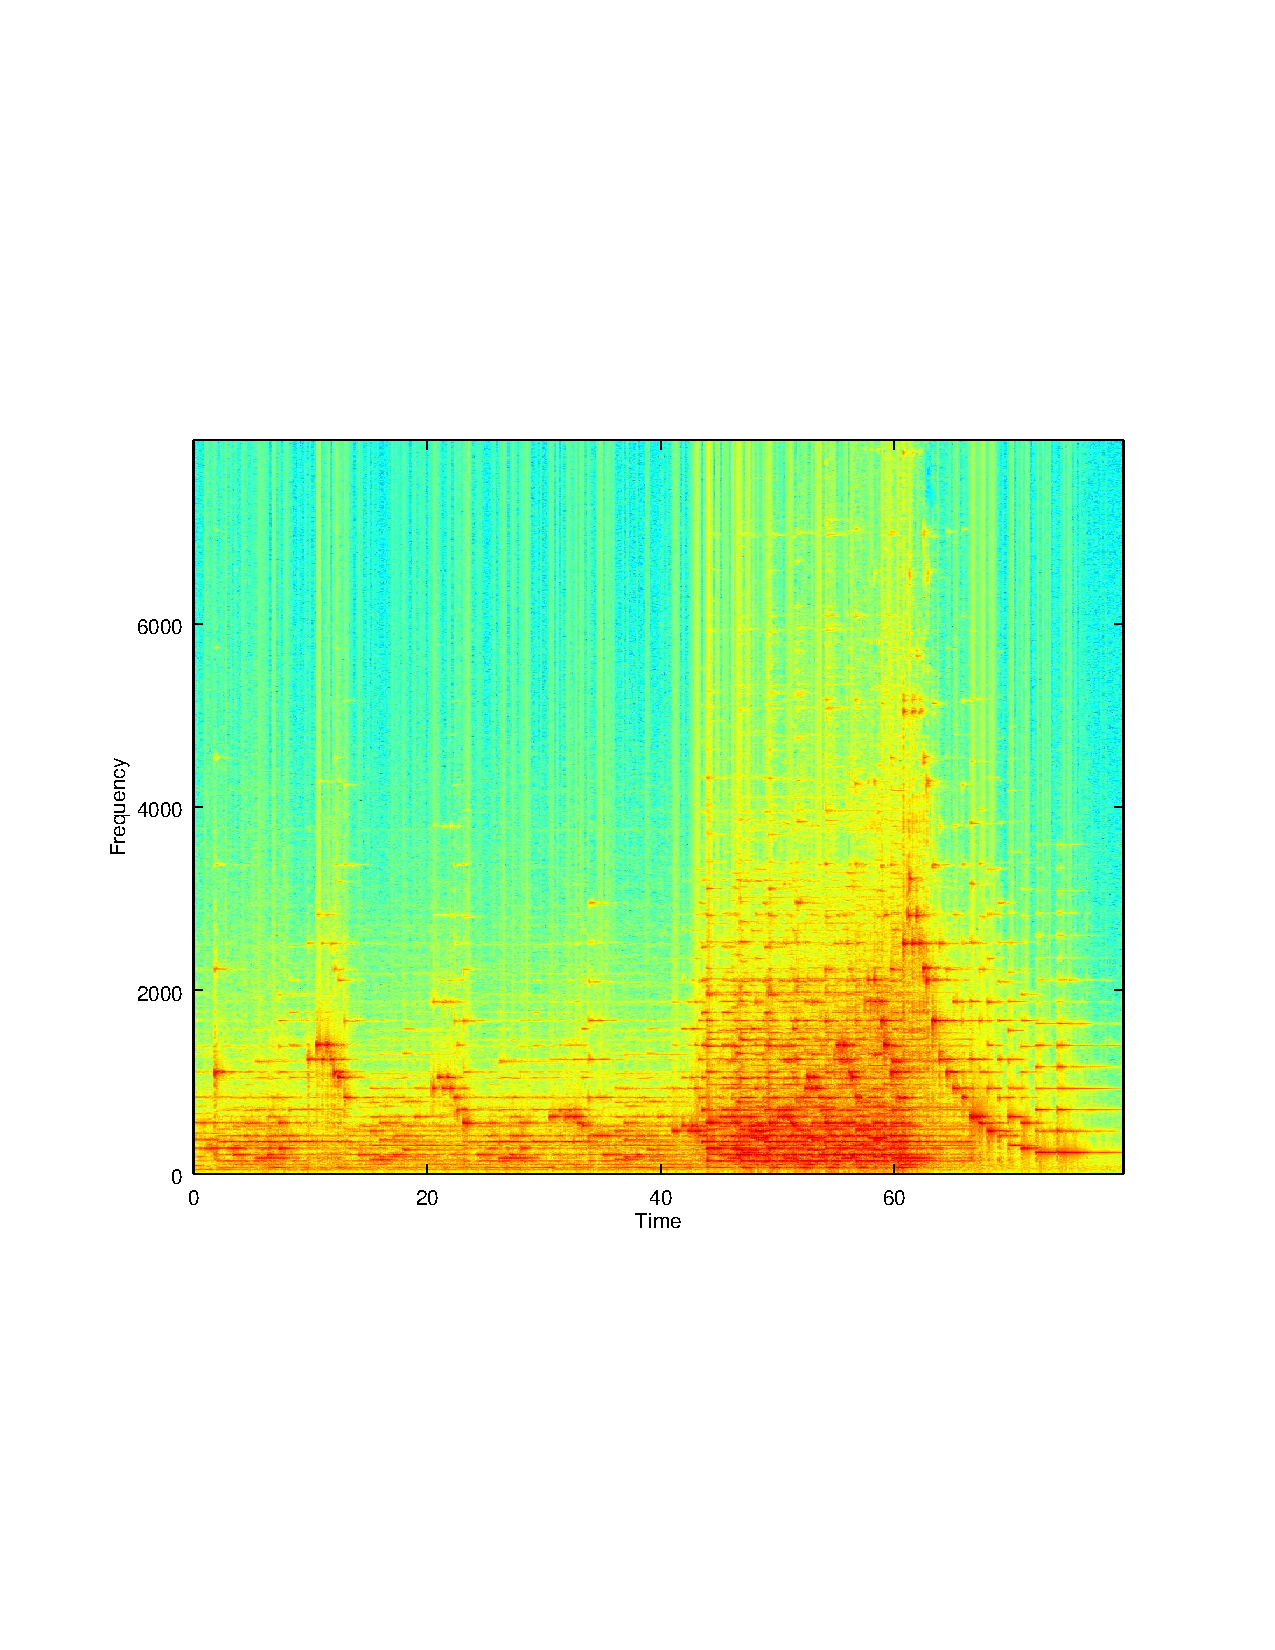
\includegraphics[width=\textwidth]{../images/specgram_6_interpolated.pdf}
\caption{Espectrograma del audio interpolado espectralmente}
\label{audio_interpolado_espectralmente}
\end{figure}

En este ejercicio, utilizando la función de síntesis del anterior punto, realizamos la misma idea que en el punto 3 pero esta vez interpolando el espectrograma, con la esperanza de obtener una canción que sea el doble de larga pero con el mismo espectro que la original.

Lamentablemente, si bien el grueso energía del espectro se mantiene en las mismas frecuencia (es decir, son las mismas notas) en el proceso de síntesis se agregan artefactos de alta frecuencia que no supimos cómo remover. Estimamos que dichos artefactos se producen ya que no ``empalmamos'' adecuadamente los distintos segmentos de la señal.


\section{Ejercicio 7}

Análogamente a lo hecho en el ejercicio 4, queremos acortar el audio a la mitad pero esta vez manteniendo el contenido espectral. Para ello, aplicamos la reconstrucción sobre una decimación de orden 2 del espectro.

De la misma manera que nos ocurrió en el ejercicio anterior, si bien mantenemos el grueso de la energía en la misma zona de frecuencias, tenemos muchos artefactos (que suenan como un ``traqueteo'') que no pudimos resolver. Podemos observar el espectrograma en \ref{audio_decimado_espectralmente}

\begin{figure}[b!]
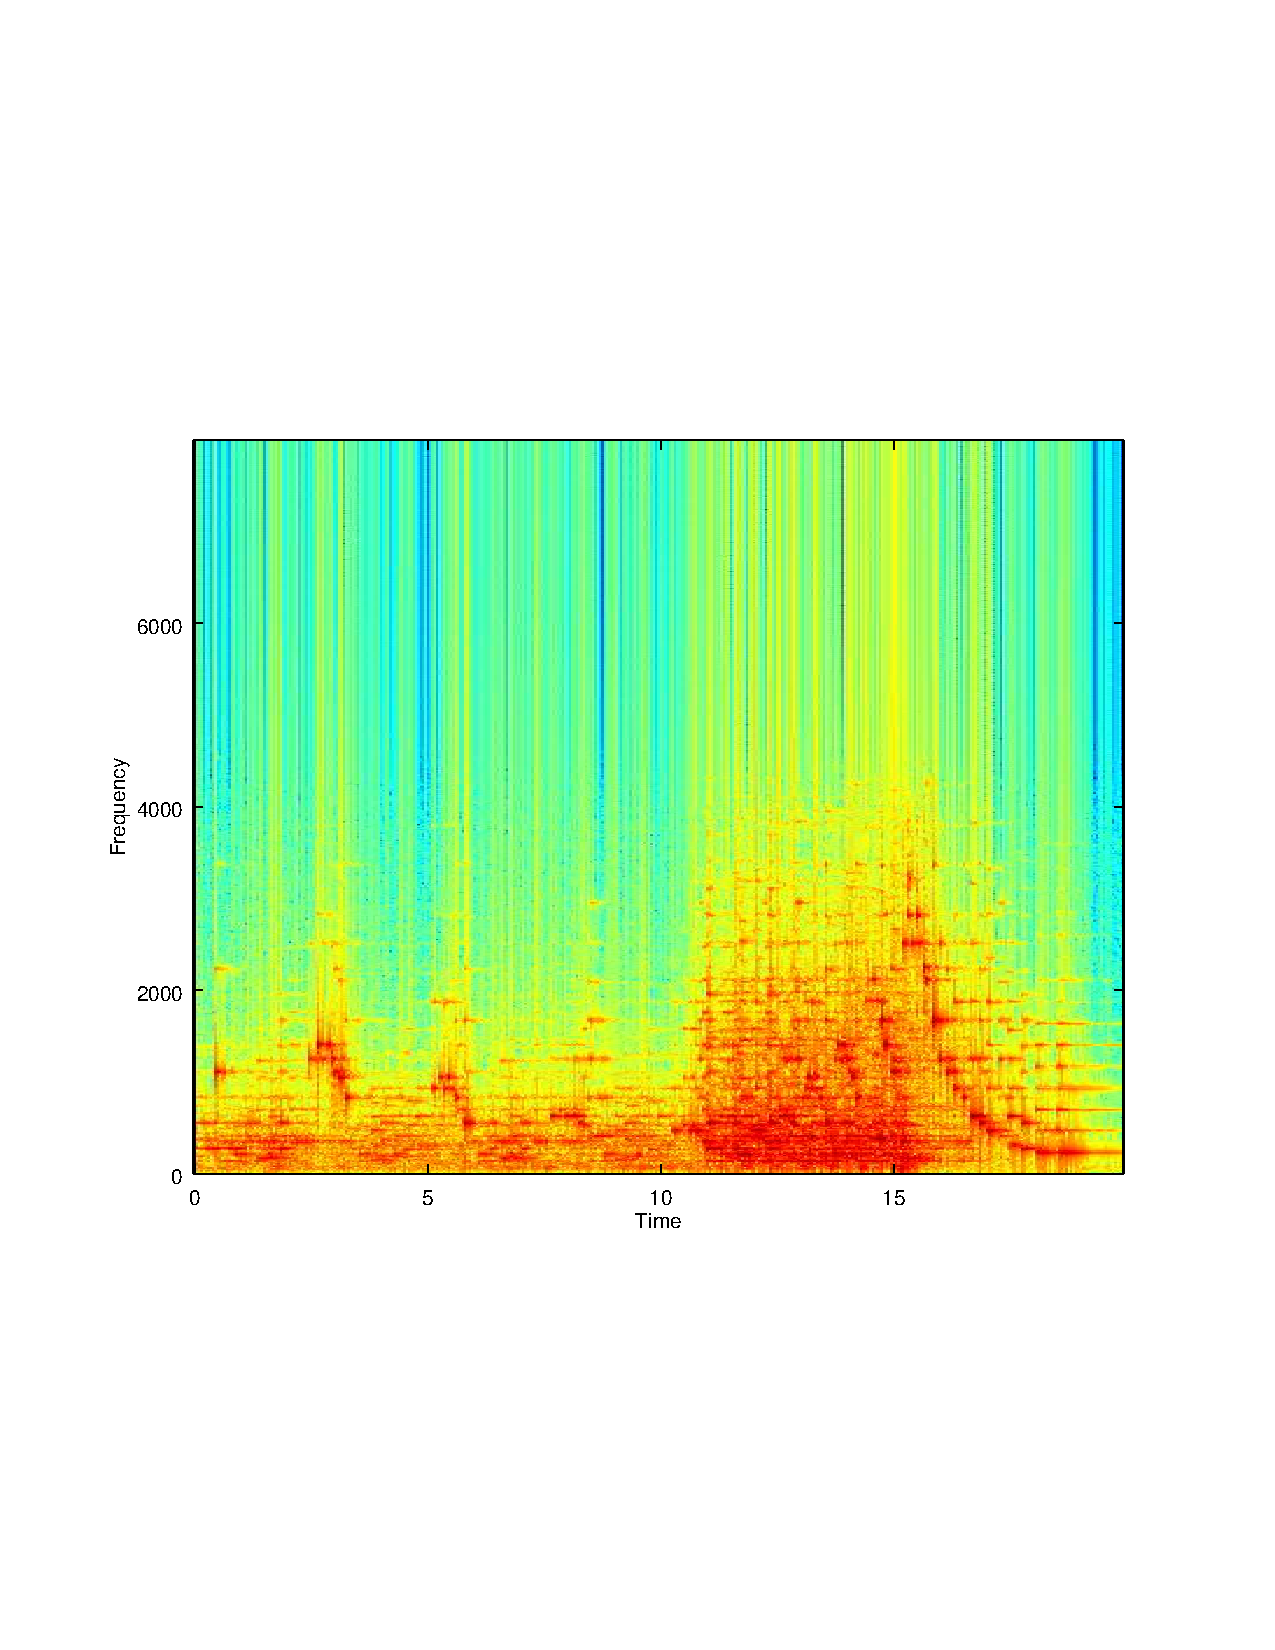
\includegraphics[width=\textwidth]{../images/specgram_7_decimated.pdf}
\caption{Espectrograma del audio decimado espectralmente}
\label{audio_decimado_espectralmente}
\end{figure}
\end{document}